
\chapter{SSH connection with the GCS} \label{app:ssh}

Assuming that the steps in Appendix \ref{app:network} were successfully completed, this Appendix explains how to obtain the parameters needed to set up the SSH connection between the OCAS and the GCS.

\begin{enumerate}
	\item Open a Command Prompt window as Administrator (network commands cannot be run by regular users for safety reasons)

	\item Check that the Raspberry Pi's MAC address by showing the devices that are connected to the Windows' network:

		\hspace{0.05\textwidth}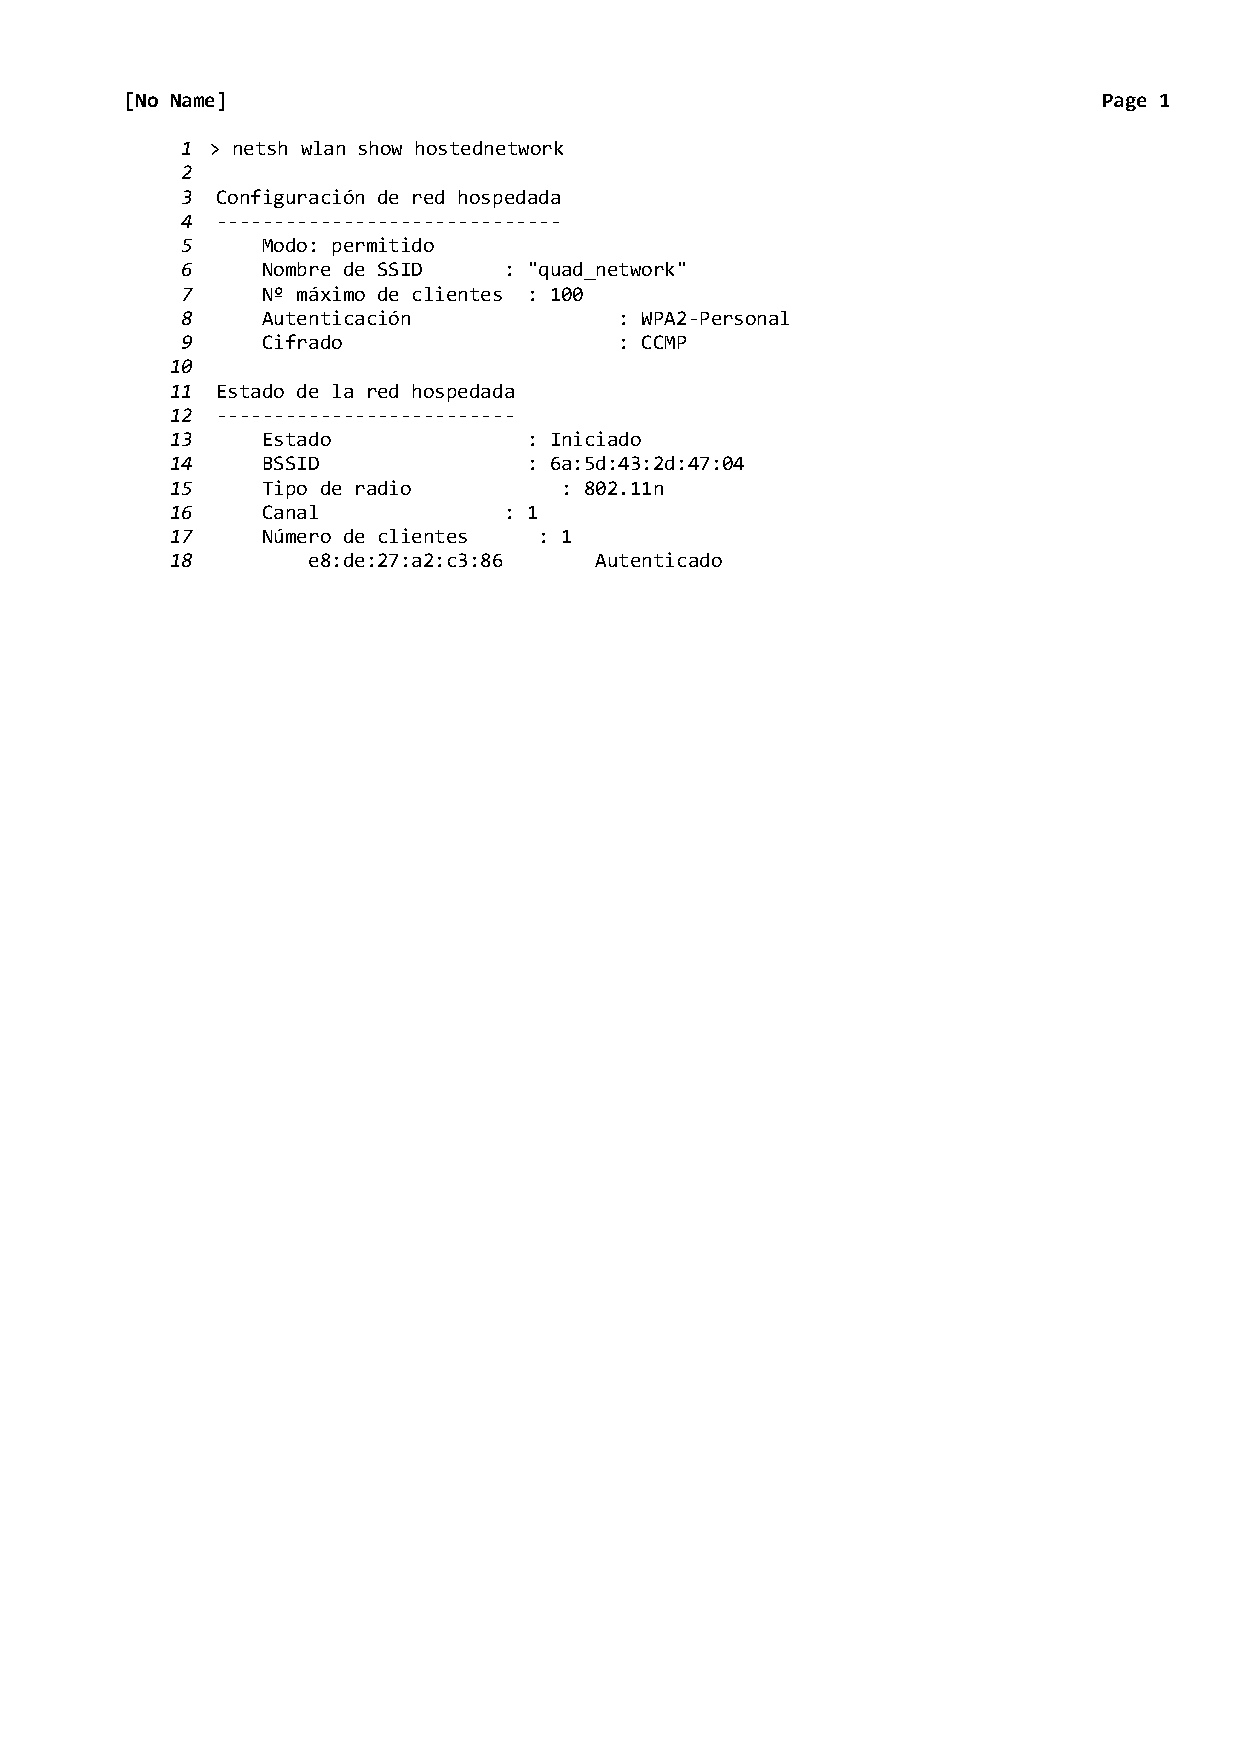
\includegraphics[width=0.95\textwidth,clip,trim={3.5cm 20cm 0 2.3cm}]{./files/shownetwork.pdf}

		In this case the Raspberry Pi's MAC address is \texttt{e8:de:27:a2:c3:86}

	\item Match the MAC address to the assigned IP given by the DHCP server

		\hspace{0.05\textwidth}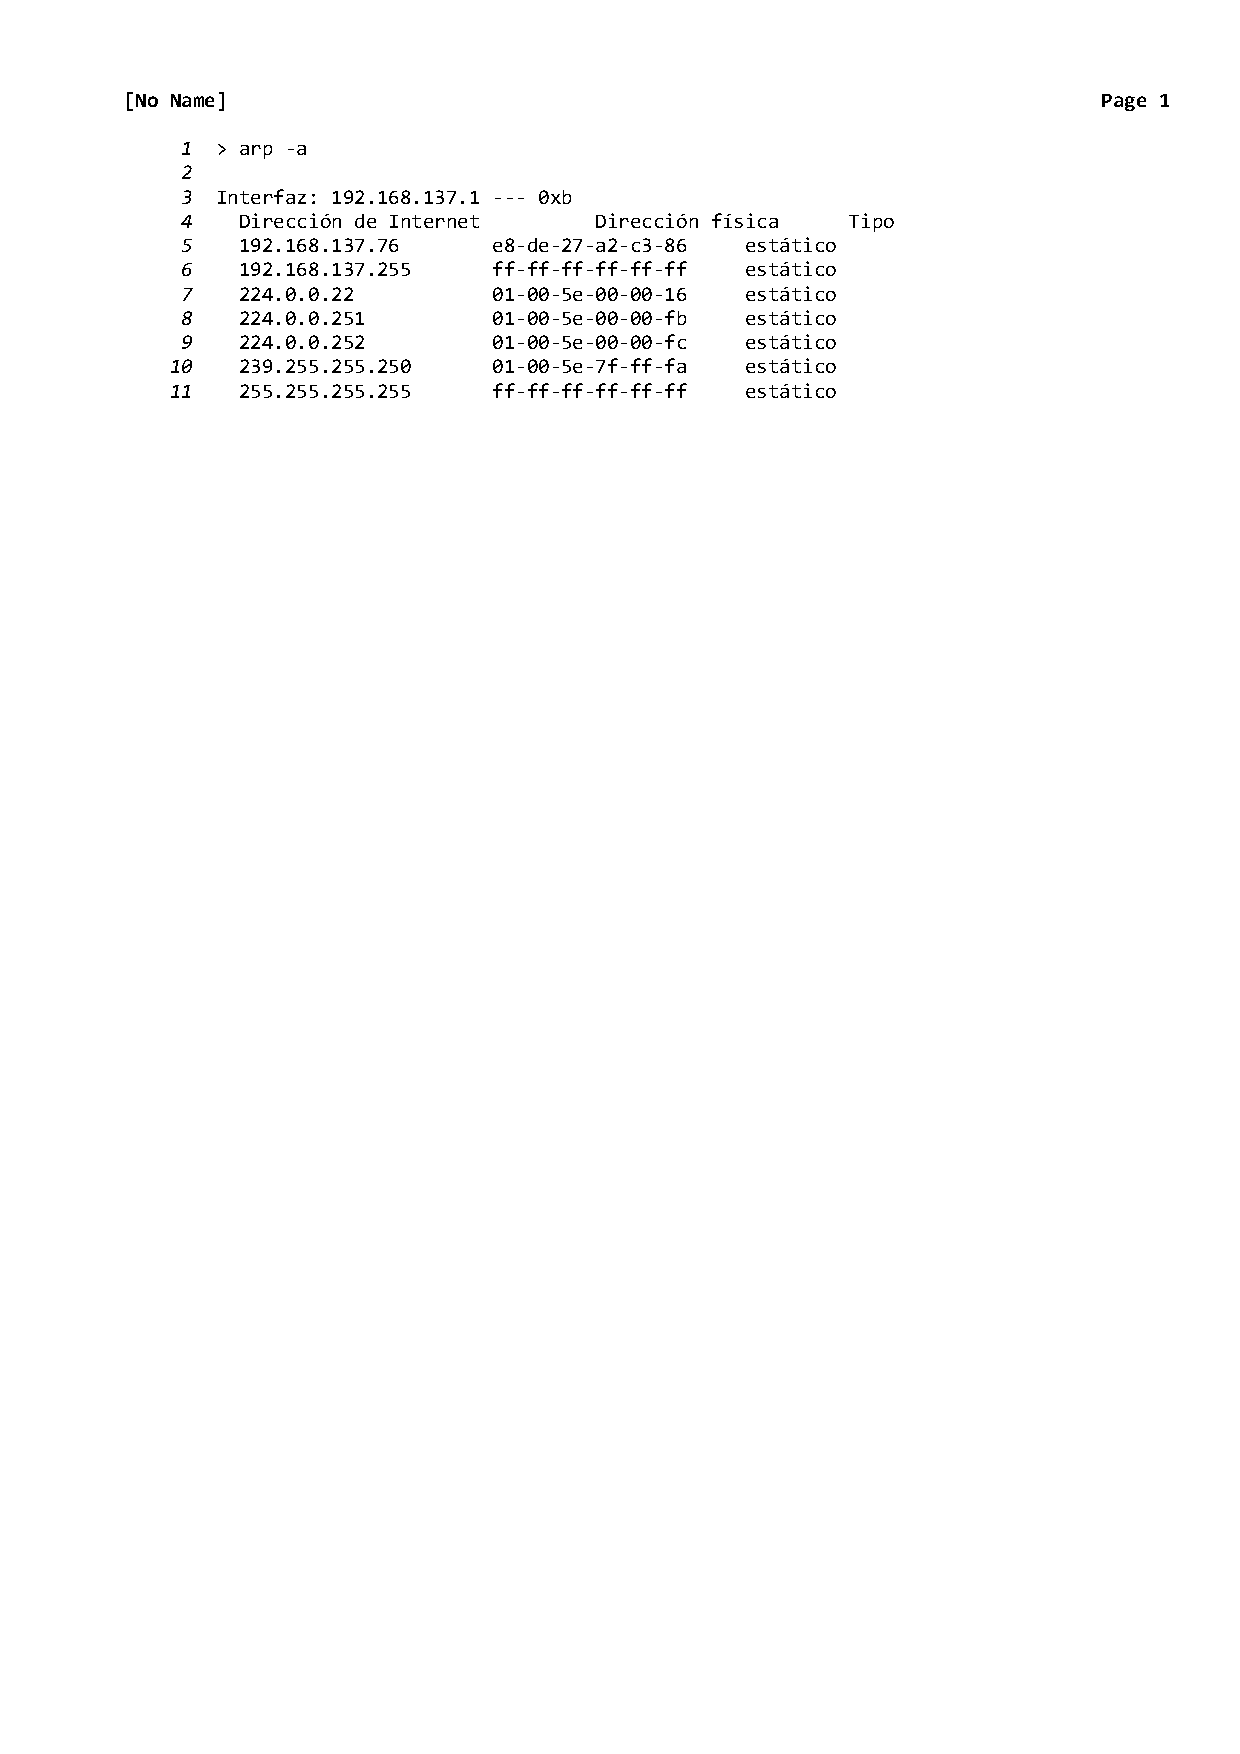
\includegraphics[width=0.95\textwidth,clip,trim={3.5cm 22.8cm 0 2.3cm}]{./files/arpnetwork.pdf}

		If the ARP cache is cluttered and the MAC address cannot be found, a flush might be helpful to clear unused entries:

		\hspace{0.05\textwidth}
\includegraphics[width=0.95\textwidth,clip,trim={3.5cm 27cm 0 2.3cm}]{./files/flusharp.pdf}

		In the example, the Raspberry Pi has been assigned the IP \texttt{192.167.137.76}

	\item To make use of the SSH protocol (being the 22$^{nd}$ port the one reserved for SSH communications) from a Windows machine, third party software is required.

		PuTTY is the most common option for all types of network communication, but can be slightly limited for the operation of the OCAS

		\begin{center}
			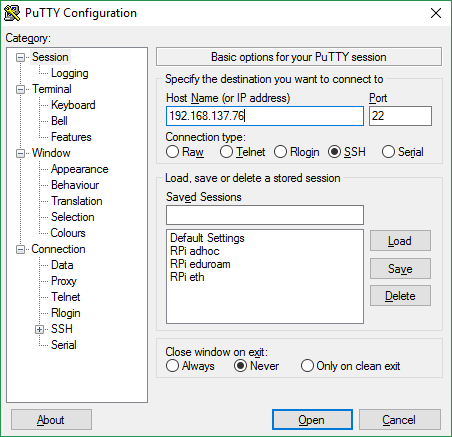
\includegraphics[width=0.6\textwidth]{./files/putty.png}
		\end{center}

		However, there exist more powerful alternatives to PuTTY, such as MobaXterm, which apart from SSH communications, can also handle X Window System forwarding; useful for the execution of graphical application directly on the Raspberry Pi, mirroring the interface on the Windows machine

		\begin{center}
			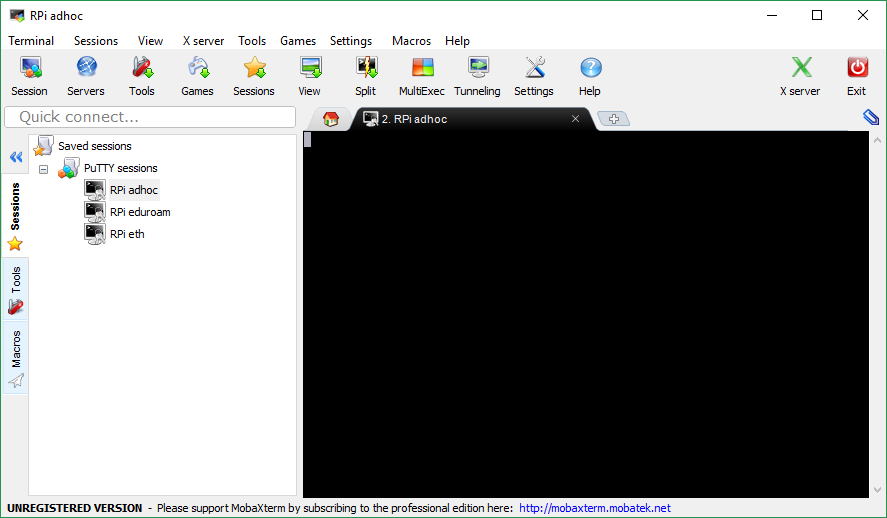
\includegraphics[width=0.8\textwidth]{./files/moba.png}
		\end{center}

	\item After connecting to the Raspberry Pi, user will be prompted to type the username and password. The default values are:

		\hspace{0.05\textwidth}
\includegraphics[width=0.95\textwidth,clip,trim={3.5cm 26.5cm 0 2.3cm}]{./files/password.pdf}

	\item From this point the user will have complete access to the Linux system, in the same way as if they were operating directly from a terminal window

\end{enumerate}
